\documentclass[tikz,border=0pt]{standalone}
\usepackage[T1]{fontenc}
\usepackage{helvet}
\renewcommand{\familydefault}{\sfdefault}
% Reuse accepted label-free artwork through vector viewports; no pixel editing.
\usepackage{graphicx}
\usetikzlibrary{arrows.meta,calc}
\tikzset{flow/.style={-{Stealth[length=1.6mm,width=1.1mm]},line width=.5pt},
 every node/.style={font=\fontsize{9}{11}\selectfont,align=center,inner sep=1pt}}
% Arguments: source left/top/right/bottom pixels; destination left/bottom/width mm.
\newcommand{\artpiece}[7]{
 \pgfmathsetmacro{\pieceScale}{#7/((#3-#1)*.1)}
 \begin{scope}[shift={(#5,#6)},scale=\pieceScale,transform shape]
  \clip (0,0) rectangle ({(#3-#1)*.1},{(#4-#2)*.1});
  \node[anchor=south west,inner sep=0pt] at ({-#1*.1},{-(931-#4)*.1})
   {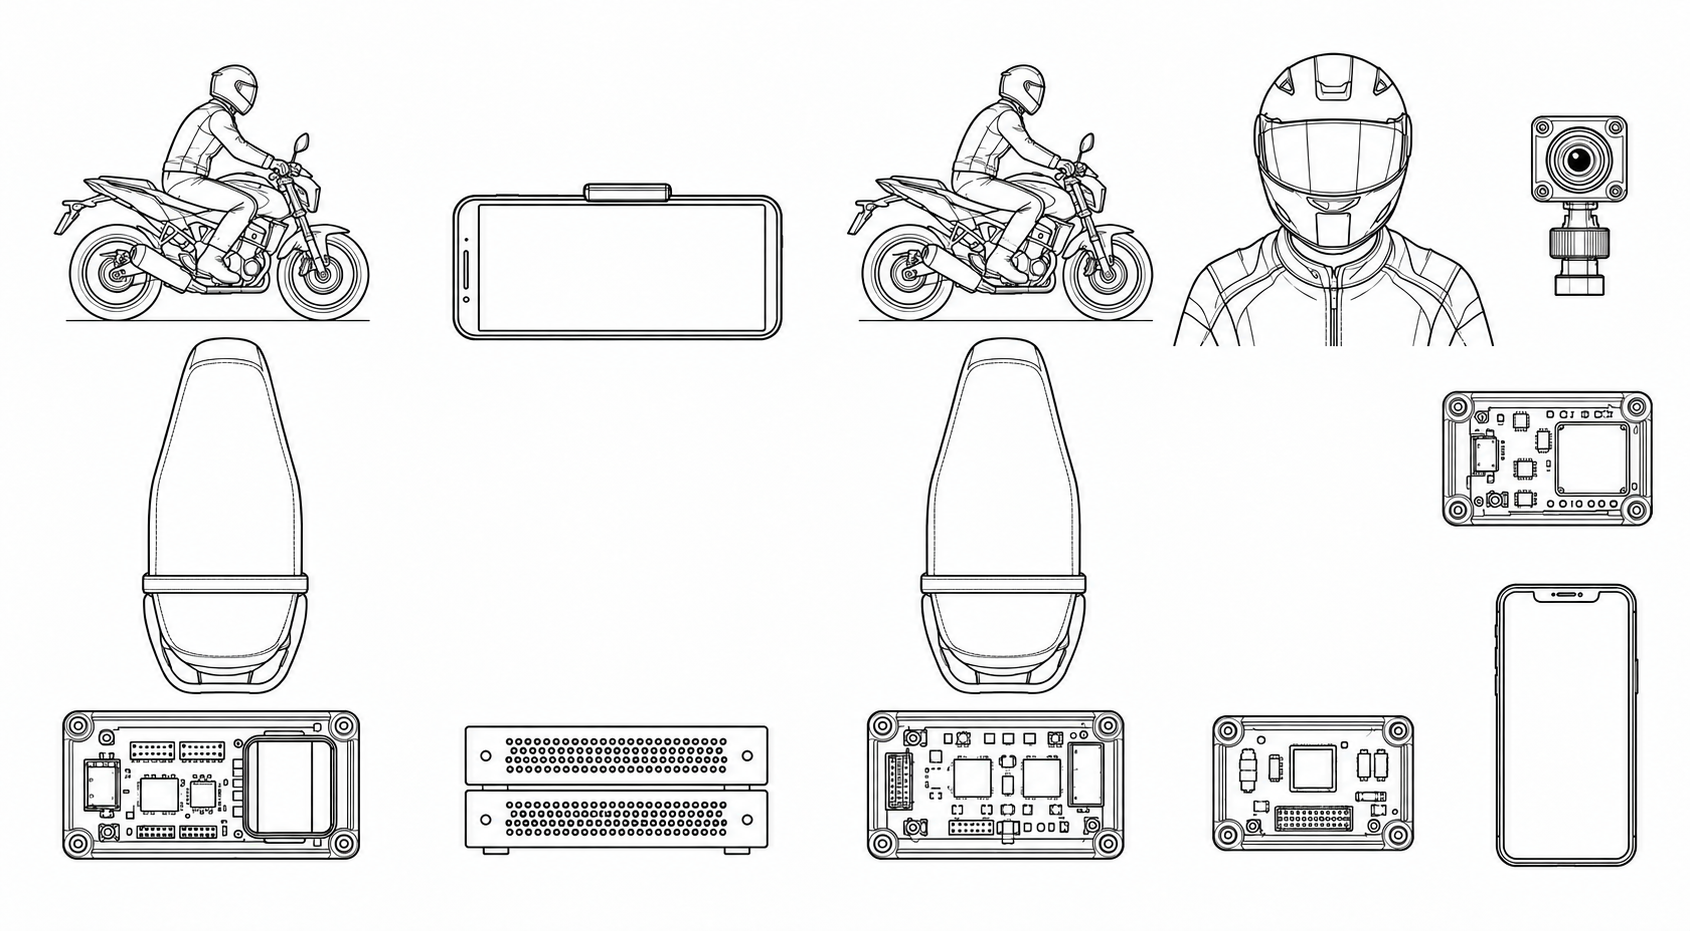
\includegraphics[width=169mm]{../reride/artwork-original.png}};
 \end{scope}}
\newcommand{\marker}[2]{
 \fill[white] (#1-2.4,#2-2.4) rectangle (#1+2.4,#2+2.4);
 \fill (#1-2,#2-2) rectangle (#1+2,#2+2);
 \fill[white] (#1-1.2,#2-1.2) rectangle (#1+1.2,#2+1.2);
 \fill (#1-1.2,#2-1.2) rectangle (#1,#2);
 \fill (#1,#2) rectangle (#1+1.2,#2+1.2);
}
\newcommand{\phoneglyph}[2]{
 \begin{scope}[shift={(#1,#2)}]
  \draw[densely dotted] (-8,0)--(8,0) (0,-13)--(0,13);
  \draw (0,10) .. controls (7,12) and (3,4) .. (7,-1)
    .. controls (11,-9) and (-4,-13) .. (-6,-7)
    .. controls (-9,0) and (-6,8) .. (0,10);
 \end{scope}}

\begin{document}
\begin{tikzpicture}[x=1mm,y=1mm,line width=.4pt,line cap=round,line join=round]
\path[use as bounding box] (0,0) rectangle (240,180);
\node at (120,171) {Complementary sensing for glanceable on-ride posture feedback};
\artpiece{1170}{45}{1500}{345}{8}{108}{53}
\marker{34.5}{149.2}\marker{34.5}{126.3}\marker{16.8}{117.7}\marker{53.5}{117.7}
\node at (35,102) {4 upper-body fiducials};
\artpiece{1520}{110}{1640}{302}{77}{132}{20}
\node at (86,124) {Camera};
\draw[flow,dashed] (77,149)--(61,149);
\artpiece{1435}{384}{1660}{535}{108}{132}{38}
\node at (127,123) {Camera Pi};
\draw[flow] (97,145)--(108,145);
\artpiece{130}{330}{315}{700}{17}{40}{25}
\foreach \yy in {58,67,76}{\foreach \xx in {25,33}{\draw[fill=white] (\xx,\yy) circle (1.4);}}
\node at (29,32) {6 pressure sites};
\artpiece{860}{707}{1135}{865}{84}{49}{44}
\node at (106,39) {Seat Pi + 2 ADCs};
\draw[flow] (42,62)--(84,62);
\artpiece{1200}{708}{1425}{862}{155}{86}{40}
\node at (175,78) {Central processing};
\draw[flow] (146,145)--(175,145)--(175,113.4);
\draw[flow] (128,62)--(175,62)--(175,86);
\node at (163,69) {WebSockets};
\artpiece{1490}{580}{1645}{868}{204}{80}{28}
\phoneglyph{218}{106}
\node at (218,72) {Glanceable posture};
\draw[flow] (195,99)--(204,99);
\draw (8,27)--(232,27);
\node at (120,20) {BANk separates sensing, processing and display modules};
\node at (120,9) {Modules explored; full integration, ride-data evaluation and LSTM learning are future work};
\end{tikzpicture}
\end{document}
